\documentclass[11pt,a4paper]{article}

% ------ PACKAGES ------

\usepackage[utf8]{inputenc}%encodage en utf8
\usepackage[english]{babel} %permet caractères français
\usepackage[T1]{fontenc} %permet cararct spéciaux
\usepackage{hyperref}  %liens hypertextes

\usepackage{array}
\usepackage{float}
\usepackage{lscape}

\usepackage{amsmath,amsthm} %pour les maths
\usepackage{commath}
\usepackage{setspace}%pour avoir un inteligne de 1.5

\usepackage{multirow}  %Tableaux à plusieurs lignes

\usepackage{geometry}%réglages mise en page
\usepackage{fancyhdr}%for headers and footers
\pagestyle{fancy}
\usepackage{algorithm}
\usepackage{algorithmic}
\usepackage{optidef} %formules d'optimisation

\usepackage{parskip}

\newtheorem{theorem}{Theorem}
\newtheorem{defn}[theorem]{Definition}
\newtheorem{example}[theorem]{Example}
\newtheorem{remark}[theorem]{Remark}
\newtheorem{question}[theorem]{Question}

\newtheorem{lemma}[theorem]{Lemma}
\newtheorem{claim}[theorem]{Claim}
\newtheorem{prop}[theorem]{Proposition}
\newtheorem{corollary}[theorem]{Corollary}
\newtheorem{conjecture}[theorem]{Conjecture}

\newtheorem{hyp}[theorem]{Hypothesis}

\onehalfspacing   %interligne de 1.5

\renewcommand{\algorithmicrequire}{\textbf{Input:}}
\renewcommand{\algorithmicensure}{\textbf{Output:}}

% ------ ADD SUBSUBSECITONS ------
\setcounter{secnumdepth}{3}
\setcounter{tocdepth}{3}

% ------ PAGE LAYOUT ------
\geometry{
%a4paper
%body={170mm,260mm},
left=35mm, top=25mm,
bottom=25mm, right=25mm
%headheight=10mm, headsep=10mm,
%footskip=10mm
}

% ---------- COMMAND SETTERS -----------

\newcommand{\HRule}{\rule{\linewidth}{0.5mm}} %newcommand for cover page

\begin{document}
\begin{titlepage}
\begin{center}

\textsc{\LARGE universit\'e libre de bruxelles}\\[2.5cm]

% Upper part of the page. The '~' is needed because \\
% only works if a paragraph has started.

\includegraphics[width=0.3\textwidth]{Images/ulblogo.jpg}~\\[1cm]

\textsc{\Large  TRAN-F501 \\[0.3cm] Internship - 201819 }\\[0.5cm]

% Title
\HRule \\[0.6cm]
{ \huge \bfseries Project:
A stochastic simulation system for protein aggregation \\[0.6cm] }

\HRule \\[2cm]

% Author and supervisor

\begin{center} \large
\emph{Supervisor:} \\
Tom \textsc{Lenaerts}\\


\emph{Author:}\\
Prateeba\textsc{ Ruggoo}\\
\end{center}

\vfill

% Bottom of the page
{\large \today}

\end{center}
\end{titlepage}


\tableofcontents \pagebreak

\section{Introduction}
Diseases like Alzheimer and Parkinson disease are the result of proteins aggregating into large fractal structures that hinder the cell function or even destroy them. Understanding how aggregates are formed and change over time is important to understand when they become harmful and how maybe treatments affect aggregate formation.

The goal of this Internship is to implement a simulation system to study aggregation between proteins. This work is performed in collaboration with the Switch lab in the KU Leuven, who has an extensive expertise in studying aggregation and related diseases.

\section{First 2 weeks (12th-23rd August)}
During the first week of the Internship, I spent the first few days getting used to the work environment, did my computer and office set up, got to know my team mates and the routines (lunch time, group lunches etc) and some paperwork so that I was given access to IB2 on a daily basis.
Once I settled down, I researched the subject and mostly did a state of the art  to have a baseline knowledge.

\section{Third week (26th-31st August)}
Having acquired a basic understanding, during the third week,  I refined my reasearch and focused on the specific papers discussing the problem in order to have a deeper understanding of the theory before starting any kind of implementation.
The papers I focussed on are the following \cite{gillespie_general_1976}, \cite{meisl_molecular_2016}, \cite{gibson_efficient_2000}, \cite{jonsson_monte_2012}.

\section{Fourth week (2nd-6th September)}
The goal of this week was to implement a simple prototype (in python for now) of an exact numerical simulation method to simulate trajectories of discrete, stochastic systems.

\subsection{Gillespie's stochastic framework of chemical kinetics}
The principle task is to develop a method for simulating the time evolution of the $N$ quantities $\{X_{i}\}$, knowing only their initial values $\{X_{i}^{(0)}\}$, the form of the $M$ reactions $\{R_{\mu}\}$ and the values of the reaction parameters $\{c_{\mu}\}$.

\begin{defn}{Problem definition:}
We are given a volume $V$ containing molecules of $N$ chemically active species $S_{i}(i = 1, \dots, N)$. Let $X_{i} \equiv$ current number of molecules of chemical species $S_{i} \in V, (i = 1, 2, \dots, N)$ and let $R_{\mu} (\mu = 1, \dots, M)$ be the chemical reactions in which the species $S_{i}$ can participate where each reaction $R_{\mu}$ is characterized by a numerical reaction parameter $c_{\mu}$ and let $R$ be the different type of reactions :
\begin{gather}
  {* \rightarrow reaction products}  \\
  {S_{j} \rightarrow reaction products} \\
  {S_{j} + S_{k} \rightarrow reaction products}\\
  {2S_{j} \rightarrow reaction products} \\
  {S_{i} + S_{j} + S_{k} \rightarrow reaction products}\\
  {S_{j} + 2S_{k} \rightarrow reaction products} \\
  {3S_{j} \rightarrow reaction products}
\end{gather} , the goal is to simulate the trajectories of the $N$ chemically active species $S_i.$ and predict which reaction will occur at each time step according to the correct probability distribution.
\end{defn}

\begin{hyp}{}
The reaction parameter $c_{\mu}$ can be defined as follows : $c_{\mu} \delta t \equiv $ average probability that a particular combination of $R_{\mu}$ reactant molecules will react accordingly in the next time interval $\delta t$ (first order).
\end{hyp}

\begin{defn}State of the system is defined by the number of molecules of each species and changes discretely whenever one of the reactions is executed. The probability that a certain reaction $\mu$ will take place in the next instant of time is given by $a_{\mu}dt + o(dt).$
\end{defn}

\subsection{Gillespie's Direct Method}
Given the problem defined above, the Gillespie's Direct Method answers two questions :
\begin{enumerate}
  \item Which reaction occurs next ?
  \item When does it occur ?
\end{enumerate}

  \subsubsection{Gillespie's Direct Method formulas}
  \begin{enumerate}
    \item Probability density $P(\mu, \tau)$ that the next reaction is $\mu$ and it occurs at time $\tau \rightarrow P(\mu, \tau)d\tau = a_{\mu}exp(-\tau \sum_{j}a_{j})d\tau$.
    \item Probability for reactions $\rightarrow Pr(Reaction = \mu) = a_{\mu} / \sum_{j}a_{j}$.
    \item Probability distribution for times $\rightarrow P(\tau)d\tau = (\sum_{j}a_{j})exp(-\tau \sum_{j}a_{j})d\tau$.
  \end{enumerate}

\subsection{Gillespie's Direct Method : Pseudo code} \ref{alg:Gillespie's Direct Method}
\begin{algorithm}[!h]                     % enter the algorithm environment
\caption{Gillespie's Direct Method}       % give the algorithm a caption
\begin{algorithmic}                       % enter the algorithmic environment
\REQUIRE $N$ chemically active species $S_i, \{X_{i}^{(0)}\}$ initial values of each specie $S_i$, the set $R$ of chemical reactions and the reaction parameter $c_{\mu}$ for each reaction.
\ENSURE Sample trajectory of a chemical process in the stochastic framework.
\WHILE{!$($simulation time exceeded$)$ }
    \STATE 1. Initialization: Set initial number of molecules in the system, set $t \leftarrow 0$.
    \STATE 2. Calculate the propensity function, $a_{i} \forall i$.
    \STATE 3. Choose $\mu$ according to the distribution in eq $5$.
    \STATE 4. Choose $\tau$ according to an exponential with parameter $\sum_{j}a_{j}$ (as in eq $6$).
    \STATE 5. Update the number of molecules to reflect execution of reaction $\mu$. Set $t \leftarrow t + \tau$.
    \STATE 6. Go to step 2.
\ENDWHILE
\end{algorithmic}
\label{alg:Gillespie's Direct Method}
\end{algorithm}

\subsection{Gillespie's Direct Method : Example}
\begin{example}{Generating a sample trajectory of a chemical process in the stochastic framework.}
    \begin{figure}[!h]
    \centering
    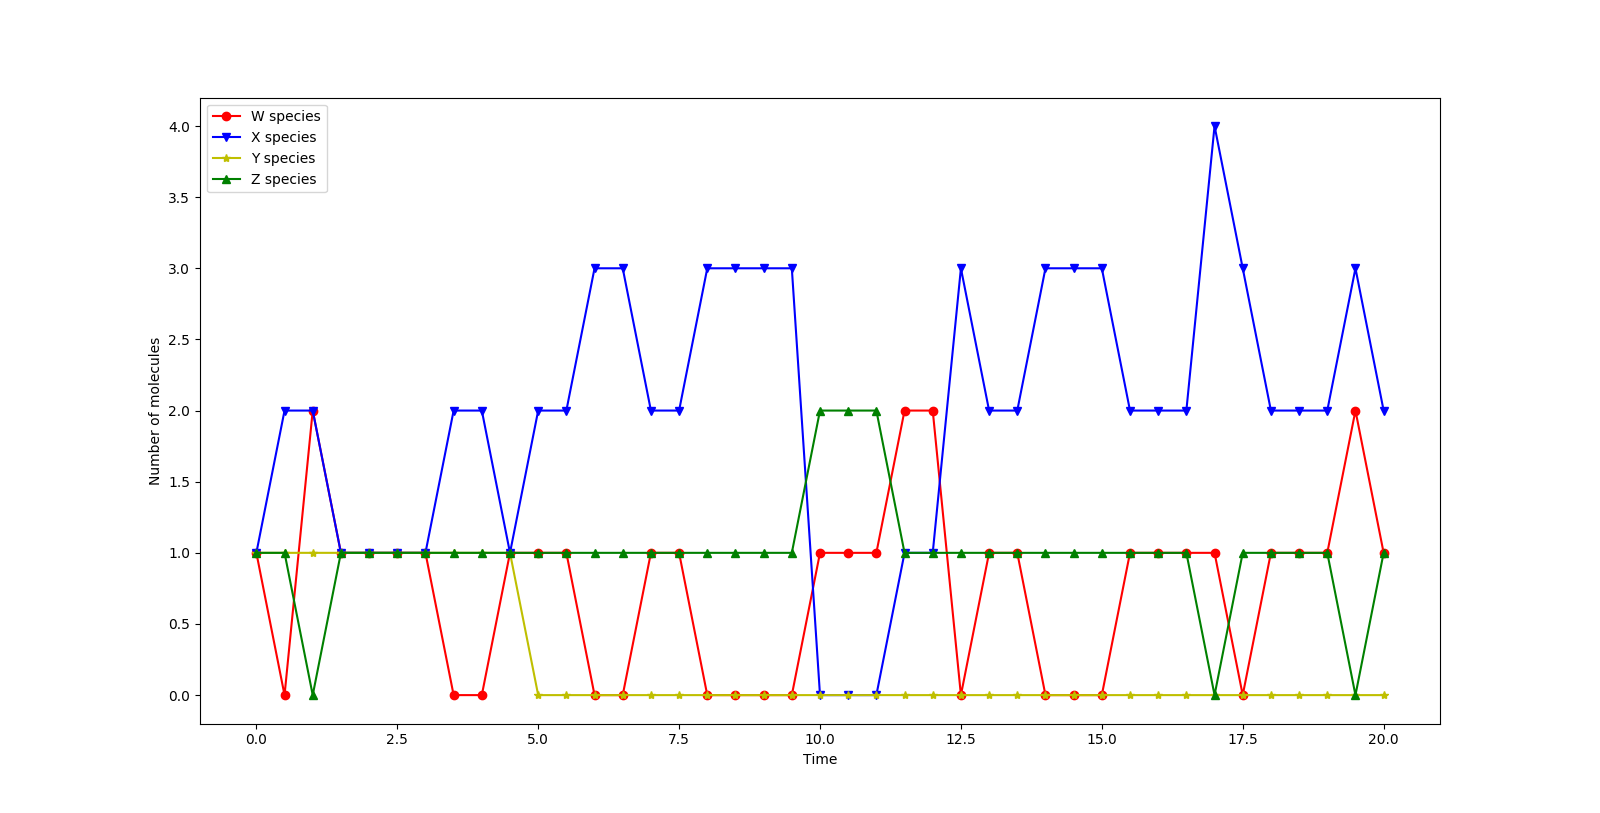
\includegraphics[width=1\textwidth]{Images/Figure_1.png}
    \caption{The x-axis denotes the duration time of the simulation and the y-axis denotes the number of molecules of each species $S_{i}$}
    \label{fig: Single sample trajectory}
    \end{figure}
\end{example}

\subsection{Gillespie's Direct Method : Implementation}
The source code of the simple simulation model can be found at To do -> put github link. The reaction set is the example used in Gillespie's paper \cite{gillespie_general_1976}.
\begin{gather}
  {X \rightarrow Y}      \\
  {Y \rightarrow X}      \\
  {2X \rightarrow Z}     \\
  {Z \rightarrow 2x}     \\
  {W + X \rightarrow 2X} \\
  {2X \rightarrow W + X}
\end{gather} and the reaction parameter $c_{\mu}$ is chosen randomly.

\section{Fourth week (9th-20th September)}
\subsection{Gillespie's Next Reaction Method}
The goal of those two weeks was to implement the Gillespie Next reaction method in order to be able to consider bigger systems. The main idea behind the Next Reaction method to generate a putative time $\tau_i$ for each reaction $i$ to occur and choose the reaction $\mu$ whose putative time $\tau_{\mu}$ is least. In order to minimize the computation time, the Next reaction method is implemented using specific data structures.

\begin{defn}
Let Reactants($\rho$) and Products($\rho$) be the sets of reactants and products of a reaction $\rho$.
\end{defn}

\begin{defn} Let $a_{\mu}$ be the value computed by the propensity function and DependsOn($a_{\mu}$) be the set of substances that affects the value $a_{\mu}$
\end{defn}

\begin{defn} Let Affects($\mu$) be the set of substances that are affected if reaction $\mu$ occurs.
\end{defn}

\begin{defn} Given a set of reactions $R$, the graph $G = G(V, E)$ is a directed graph where $V$ is the set of Reactions and there exists an edge from $v_i$ to $v_j$ if and only if  Affects($v_i$) $\cap$ DependsOn($a_{v_{j}}$) $\neq \emptyset$. $G$ is then referred to as the dependency graph of the set of reactions $R$ and is useful to know which $a_is$ to change when a given reaction occurs.
\end{defn}

\begin{defn} Indexed prioroty Queues. To do -> definition
\end{defn}

\begin{algorithm}[!h]                     % enter the algorithm environment
\caption{Gillespie's Next Reaction Method}       % give the algorithm a caption
\begin{algorithmic}                       % enter the algorithmic environment
\REQUIRE $N$ chemically active species $S_i, \{X_{i}^{(0)}\}$ initial values of each specie $S_i$, the set $R$ of chemical reactions and the reaction parameter $c_{\mu}$ for each reaction.
\ENSURE Sample trajectory of a chemical process in the stochastic framework.
\WHILE{!$($simulation time exceeded$)$ }
    \STATE 1. Initialization :
      \STATE \ \ \ 1.1  \ Set initial number of molecules, set $t \leftarrow 0$, generate a dependency graph $G$.
      \STATE \ \ \ 1.2. Calculate the propensity function, $a_{i} \forall i$.
      \STATE \ \ \ 1.3. For each $i$, generate a putative time, $\tau_{i}$, according to an exponential
      \STATE \ \ \ \ \ \ \ \ \ distribution with parameter $a_{i}$.
      \STATE \ \ \ 1.4. Store the $\tau_{i}$ values in an indexed priority queue $P.$
    \STATE 2. Let $\mu$ be the reaction whose putative time, $\tau_{\mu}$, is least.
    \STATE 3. Let $\tau$ be $\tau_{\mu}$.
    \STATE 4. Update the number of molecules to reflect execution of reaction $\mu$. Set $t \leftarrow \tau$.
    \STATE 5. For each edge($\mu$, $\alpha$) in the dependency graph $G$,
    \STATE \ \ \ \ 5.1 update $a_{\alpha}.$
    \STATE \ \ \ 5.2 if $\alpha \neq \mu$, set $\tau_{alpha} \leftarrow (a_{\alpha,old}/a_{\alpha, new})(\tau_{\alpha} - t) + t.$
    \STATE \ \ \ 5.3 if $\alpha = \mu$, generate a random number, $\rho$, according to an exponential distribution
    with parameter $a_{\mu}$ and set $\tau_{\alpha} \leftarrow \tau + t.$
    \STATE \ \ \ 5.4 Update the old $\tau_{\alpha}$ value in $P$.
    \STATE 6. Go to step $2$.
\ENDWHILE
\end{algorithmic}
\end{algorithm}

\begin{example}{Generating a sample trajectory of a chemical process in the stochastic framework.}
    \begin{figure}[!h]
    \centering
    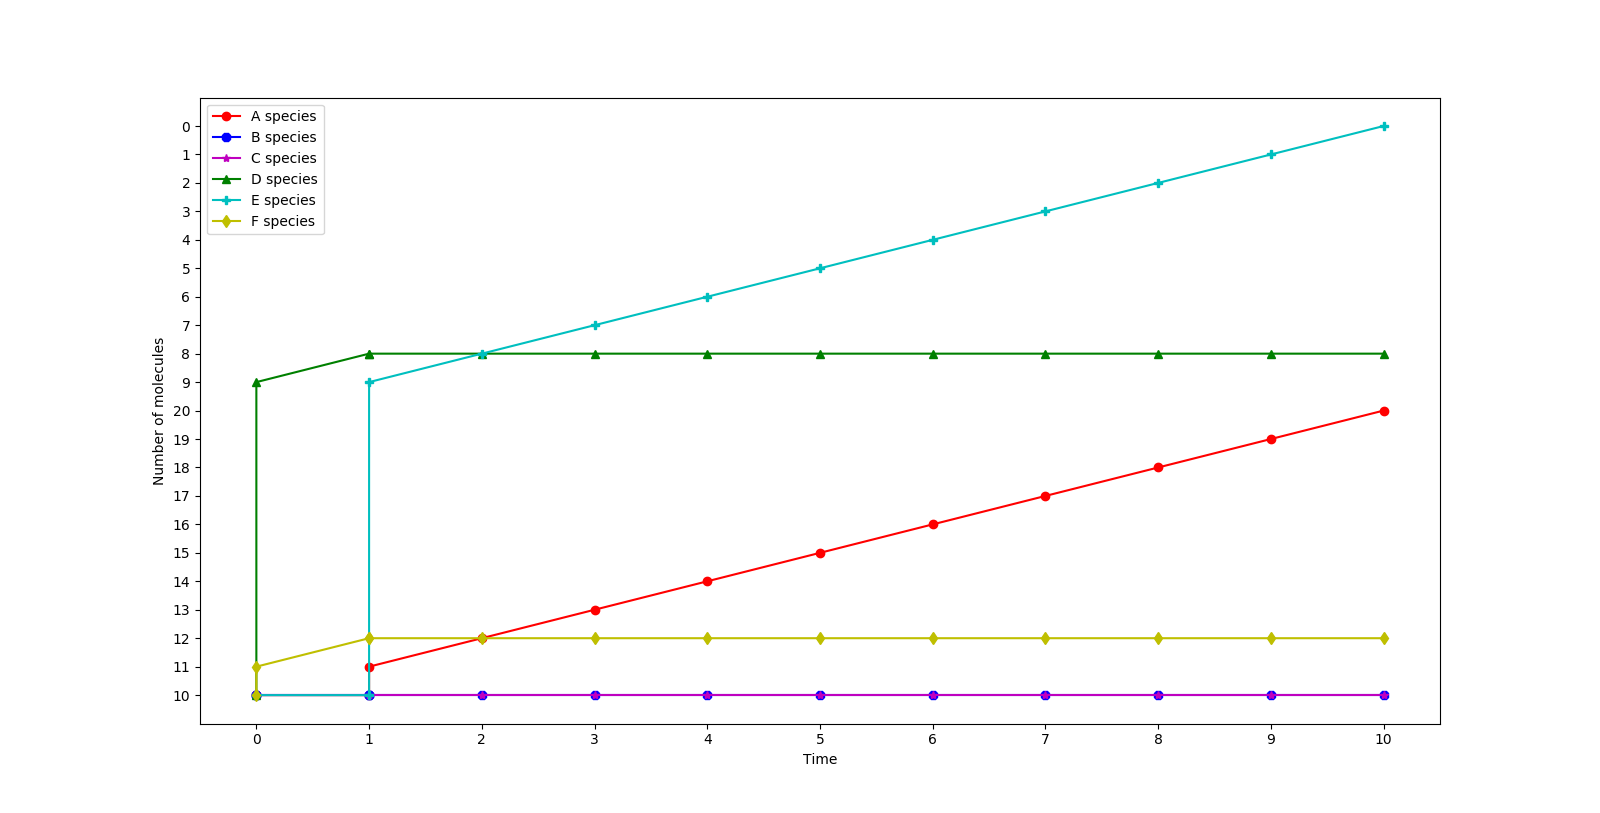
\includegraphics[width=1\textwidth]{Images/Figure_1_Next_reaction.png}
    \caption{The x-axis denotes the time used and the y-axis denotes the number of molecules}
    \label{fig: sample trajectory}
    \end{figure}
\end{example}

\begin{example}{Generating a single sample trajectory of a chemical process in the stochastic framework.}
    \begin{figure}[!h]
    \centering
    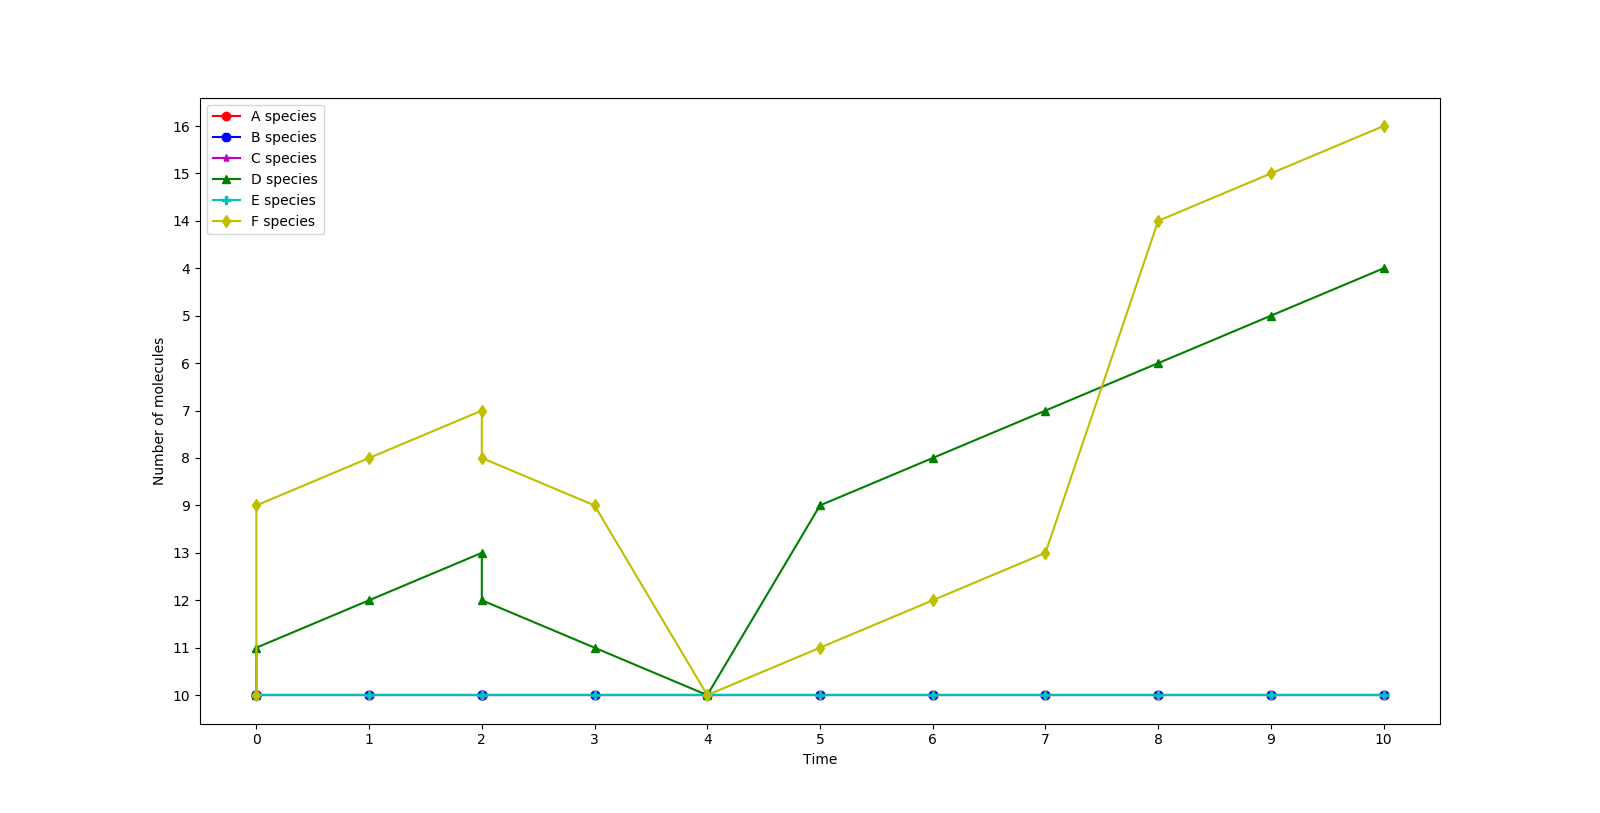
\includegraphics[width=1\textwidth]{Images/Figure_5_Next_reaction.png}
    \caption{The x-axis denotes the time used and the y-axis denotes the number of molecules}
    \label{fig: Single sample trajectory}
    \end{figure}
\end{example}

\section{Conclusion}

\newpage
\bibliographystyle{alpha}
\bibliography{combinatorial}


\end{document}
